\cleardoublepage
\thispagestyle{empty}
%\thisfancypage{\setlength{\fboxsep}{5pt}\doublebox}{}
%\setlength\intextsep{0mm}
\noindent

\includegraphics[width=0.45\textwidth]{IMG/TOP/logoVSCHT_zakl_CB.png} \\
\vspace{10mm}
\\
{\Large \textbf{Fakulta  chemicko-inženýrská}
\\ [5mm]
Ústav počítačové a řídicí techniky}

\vspace{40mm}


\begin{spacing}{0.9}
\Huge\noindent POUŽITÍ ADAPTIVNÍCH SYSTÉMŮ PŘI ANALÝZE DAT\\ 
\end{spacing}
\vspace{30mm}

\noindent
{\Large \textbf{DISERTAČNÍ PRÁCE}} 

\vspace{15mm}

\begin{table}[!h]
\begin{tabular}{  l l |l  l }
\hspace{-0.5em}AUTOR & \hspace{0mm} & & {\Large \textbf{JAN VRBA}} \\ [7mm]
\hspace{-0.5em}ŠKOLITEL &  &  & \textbf{\large JAN MAREŠ}\\ [7mm]
\hspace{-0.5em}ŠKOLITEL  SPECIALISTA             &     &   & {\textbf{\large RATACHAN}} \\ [7mm]
\hspace{-0.5em}STUDIJNÍ PROGRAM &  &  & {\large Chemické a procesní inženýrství (čtyřleté)} \\ [7mm]
\hspace{-0.5em}STUDIJNÍ OBOR    & &   & {\large Technická kybernetika}\\ [7mm]
\hspace{-0.5em}ROK          &       &   & \textbf{2020} \\
\end{tabular}


\end{table}

%===============================English============================
%=================================CZ===============================
\cleardoublepage
\thispagestyle{empty}
%=================================CZ================================
%============================English============================
\thispagestyle{empty}
\noindent

\includegraphics[width=0.45\textwidth]{IMG/TOP/logoUCT_basic_CB.png} \\
\vspace{10mm}
\\
{\Large \textbf{Faculty of Chemical Engineering}
\\ [5mm]
Department of Computing and Control Engineering}

\vspace{40mm}

\begin{spacing}{0.9}
\Huge\noindent ADAPTIVE SYSTEMS IN DATA \\ANALYSIS\\
\end{spacing}

\vspace{30mm}

\noindent
{\Large \textbf{DISSERTATION}} 

\vspace{15mm}

\begin{table}[!h]
\begin{tabular}{  l l |l  l }
\hspace{-0.5em}AUTHOR & \hspace{0mm} & & {\Large \textbf{JAN VRBA}} \\ [7mm]
\hspace{-0.5em}SUPERVISOR &  &  & \textbf{\large JAN MAREŠ}\\ [7mm]
\hspace{-0.5em}SUPERVISOR SPECIALIST    &     &   & {\textbf{\large PANÍ SOBÍKOVÁ}} \\ [7mm]
\hspace{-0.5em}STUDY PROGRAMME &  &  & {\large Chemical and Process Engineering} \\ [7mm]
\hspace{-0.5em}FIELD OF STUDY & &   & {\large Technical Cybernetics}\\ [7mm]
\hspace{-0.5em}YEAR          &       &   & \textbf{2020} \\
\end{tabular}


\end{table}

%%====================================================Declaration=====================
%\newpage
%\thispagestyle{empty}
%\vphantom{a}
%\vspace{13cm}
%\begin{figure}[H]
%\pdfimageresolution=133 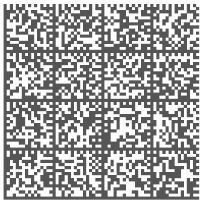
\includegraphics{IMG/TOP/QR.png}
%\end{figure}
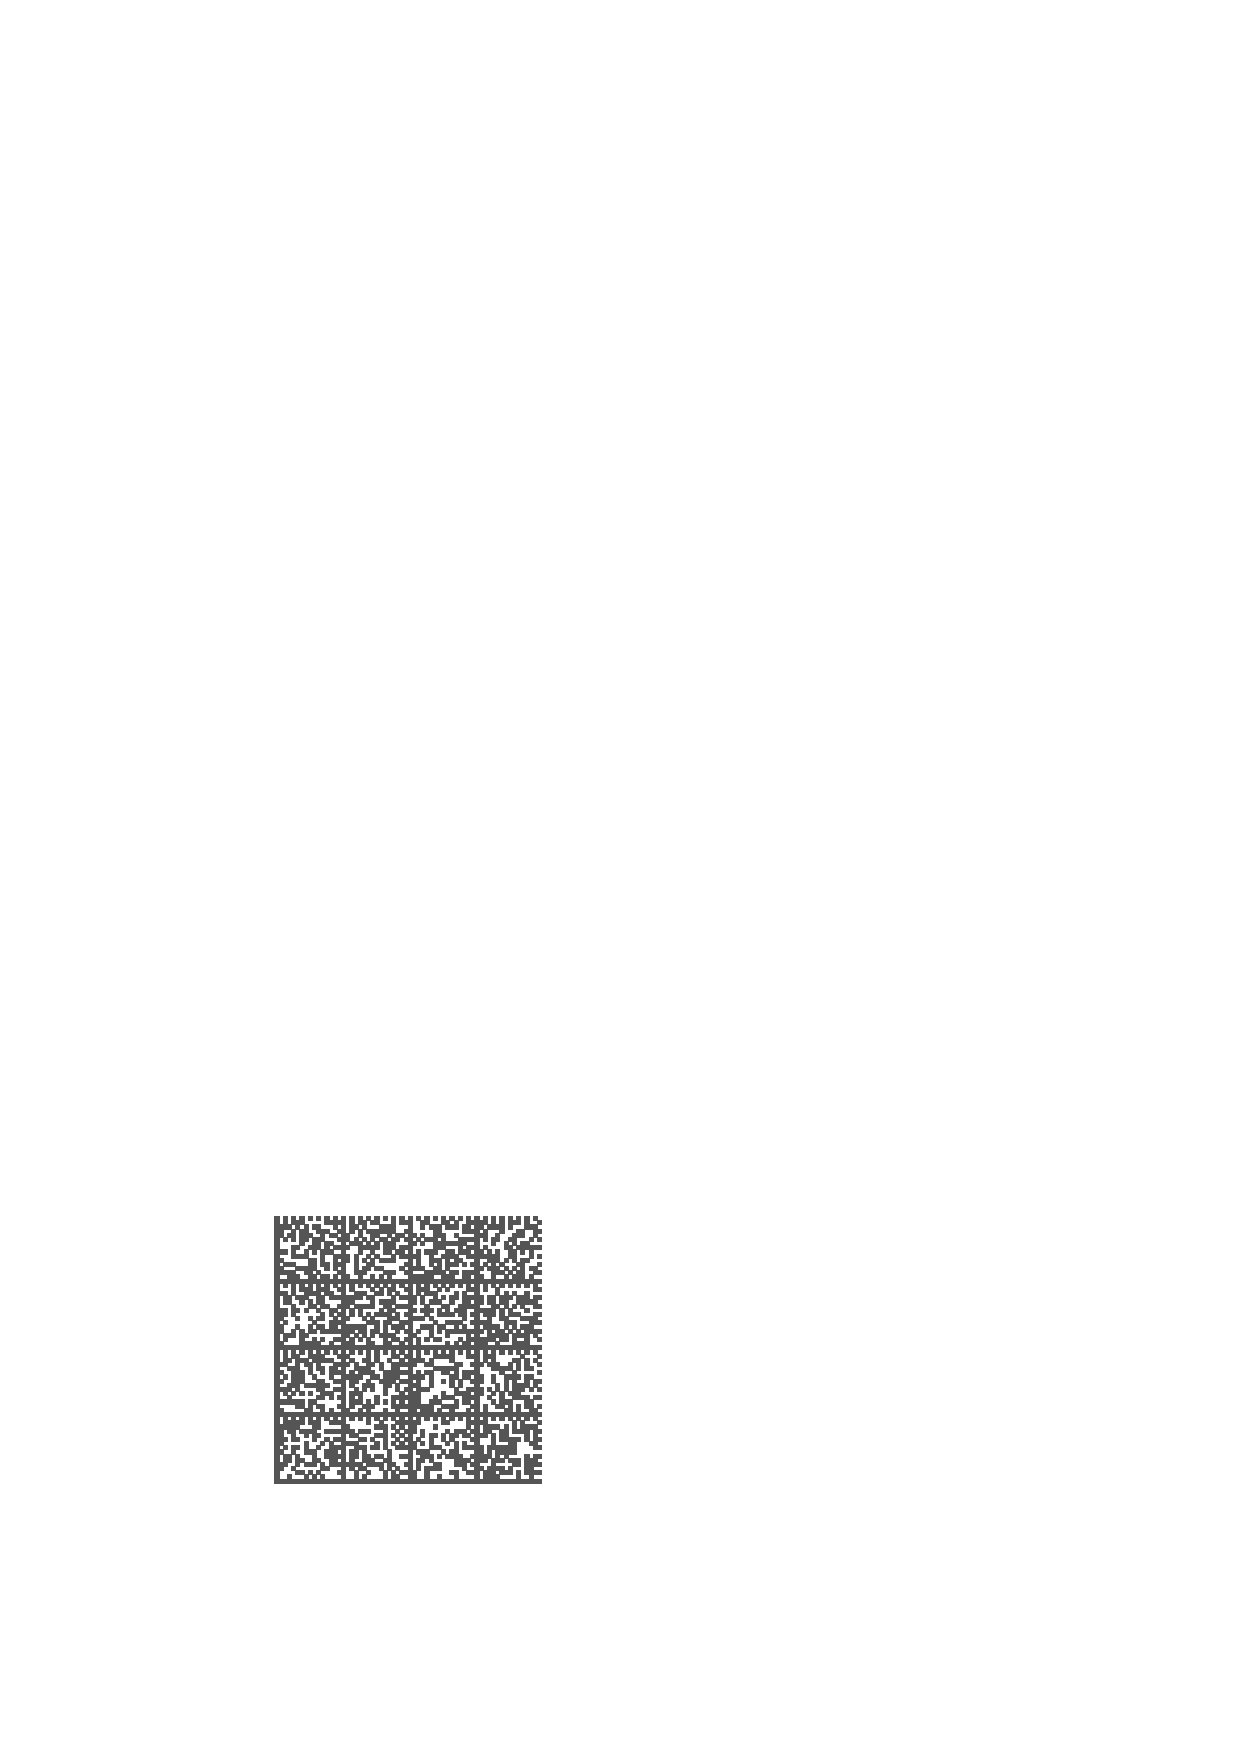
\includepdf[pages=1]{IMG/TOP/QR.pdf}
%%====================================================Declaration=====================
\clearpage
\thispagestyle{empty} 
 \vspace*{1cm}
 \noindent 
 Tato disertační práce byla vypracována na Ústavu počítačové a řídicí techniky
v období ODKDY -- DOKDY. \\ [30mm]
Prohlašuji, že jsem tuto práci vypracoval samostatně. Veškeré literární prameny
a informace, které jsem v práci využil, jsou uvedeny v seznamu použité literatury. \\ [8mm]
Byl jsem seznámen s tím, že na moji práci se vztahují práva a povinnosti vyplývající
ze zákona č. 121/2000 Sb., o právu autorském, o právech souvisejících s právem
autorským a o změně některých zákonů (autorský zákon). Zejména se jedná
o skutečnost, že Vysoká škola chemicko-technologická v Praze, popř. jiné vzdělávací
zařízení, ve kterém jsem svou práci vypracoval, má právo na uzavření licenční
smlouvy o užití této práce jako školního díla podle § 60 odst. 1 autorského zákona.
Pokud bych v budoucnu poskytl licenci o užití práce jinému subjektu, je Vysoká
škola chemicko-technologická v Praze, popř. jiné vzdělávací zařízení, ve kterém
jsem svou práci vypracoval, oprávněna ode mne požadovat přiměřený příspěvek
na úhradu nákladů, které na vytvoření díla vynaložil a to podle okolností až do
jejich skutečné výše. \\ [8mm]
\noindent
Souhlasím se zveřejněním své práce podle zákona č. 111/1998 Sb., o vysokých
školách, ve znění pozdějších předpisů. \\ [30mm]


\noindent\begin{tabular}{@{}p{2.5in}p{3.in}@{}}
\hspace{1cm} V Praze dne                      &\hspace{2cm} \dotfill\\
             & \multicolumn{1}{c}{\hphantom{hhhhHHHHH}JMÉNO}\\
\end{tabular} 

 
\cleardoublepage
\thispagestyle{empty}

 \vspace*{\fill}
 \noindent {\bf \large Poděkování} \\ [5mm]
Děkuji vedoucímu mé dizertační práce doc. Ing. Janu Marešovi, Ph.D. za všestrannou pomoc, podporu a trpělivost. Děkuji doc. Ing. Ivo Bukovskému, Ph.D.  za otevření dveří do světa detekce novosti. Rád bych poděkoval také Matouši Cejnkovi za inspiraci, blahodárné diskuze a spolupráci nejen na bitevním poli světa H\&G. Děkuji všem zaměstnancům Ústavu počítačové a řídicí techniky na VŠCHT. V neposlední řadě bych chtěl poděkovat také všem přátelům, kteří mi pomohli udržet zdravou životní rovnováhu. Zvláštní poděkování patří  mým rodičům a sestře Radaně za podporu během mého dlouhého studia. Děkuji také Otovi, který mi přinesl spoustu štěstí a radosti. Nejvíce děkuji mé Kazumi za podporu, trpělivost, obětavost a za vytvoření ideálních podmínek, ve kterých jsem mohl práci psát.  

 





%-------------------------------Abstract CZ ---------------------------------------------
\cleardoublepage
\thispagestyle{empty}
%-------------------------------Abstract CZ ---------------------------------------------

\noindent {\bf \large Souhrn} \\ [5mm]
Disertační práce se zabývá detekcí novosti, zejména pak algoritmem Extreme Seeking Entropy. \#TODO \\ [5mm]
\noindent {\bf \large Klíčová slova}  \\ [5mm] \noindent {\it SLOVO}
\#TODO

\cleardoublepage
\thispagestyle{empty}


%----------------------------------------------------Abstract  English--------------------------------------------------
\cleardoublepage
\thispagestyle{empty}

\noindent {\bf \large Summary} \\ [5mm] 
This dissertation deals with \#TODO
\\ [5mm]



\noindent {\bf \large Keywords}  \\ [5mm]
{\it WORD}
\#TODO



%%v~v~v~v~v~v~v~v~v~v~v~v~v~v~v~v~v~v~v~v~v~v~v~v~v~v~v~v~v
%\thispagestyle{empty}
%%v~v~v~v~v~v~v~v~v~v~v~v~v~v~v~v~v~v~v~v~v~v~v~v~v~v~v~v~v
\cleardoublepage
\tableofcontents
\thispagestyle{empty}
%\addtocontents{toc}{~\hfill\textbf{Page}\par}
%\addcontentsline{toc}{chapter}{Contents}
%%v~v~v~v~v~v~v~v~v~v~v~v~v~v~v~v~v~v~v~v~v~v~v~v~v~v~v~v~v

%\newpage
%\setcounter{page}{1}

% Seznam zkratek
\cleardoublepage
\thispagestyle{empty}

\chapter*{Seznam použitých zkratek}
\begin{tabular}{ll}
LE                      & learning entropy                              \\
ELBND                   & error and learning based novelty detection      \\
GEV                     & generalized extreme value                       \\
GNGD                    & generalized normalized gradient descend         \\
NLMS                    & normalized least mean squares                   \\
POT                     & peak-over-threshold                             \\
LNU                     & linear neural unit                              \\
QNU                     & quadratic neural unit                           \\
SNR                     & signal-to-noise ratio                           \\
RLS                     & recursive least squares                         \\
ESE                     & extreme seeking entropy                         \\
SM-NLMS                 & set-membership normalized least mean squares \\
GPD						& generalized Paredo distribution \\
HMM						& hidden Markov model \\
GMM						& Gaussian Mixture Model \\
HONU					& higher order neural unit \\
SVM						& support vector machine \\
PCA						& principal component analysis \\
MOM						& method of moments \\
ROC						& receiver operating characteristics \\
AUROC					& area under the receiver operating characteristics\\



\end{tabular}

% Seznam zkratek
\cleardoublepage
\thispagestyle{empty}

\chapter*{Seznam symbolů}
\begin{tabular}{ll}

$\mathbb{N}$    & množina přirozených čísel                                 \\
$\mathbb{R}$    & množina reálných čísel                                    \\
$\mu$           & rychlost učení                                            \\
$\hat{y}$       & výstup adaptivního filtru                                 \\
$k$             & diskrétní časový index                                    \\
$e$             & chyba predikce                                            \\
$M_{ND}$        & délka okna pro vyhodnocení změn adaptabilních parametrů   \\
$e$             & chyba predikce                \\
$e$             & chyba predikce                \\
$e$             & chyba predikce                \\
$e$             & chyba predikce                \\
$e$             & chyba predikce                \\
$e$             & chyba predikce                \\
$e$             & chyba predikce                \\
$e$             & chyba predikce                \\
$e$             & chyba predikce                \\
$e$             & chyba predikce                \\
$e$             & chyba predikce                \\
$e$             & chyba predikce                \\
$e$             & chyba predikce                \\
$e$             & chyba predikce                \\
$e$             & chyba predikce                \\
$e$             & chyba predikce                \\
$e$             & chyba predikce                \\
$e$             & chyba predikce                \\
$e$             & chyba predikce                \\
$e$             & chyba predikce                \\
$e$             & chyba predikce                \\
\#TODO             & \#TODO              \\



\end{tabular}
